\documentclass[hidelinks,a4paper,14pt]{article}
\usepackage{ amsmath, amssymb}
\usepackage{graphicx}
\usepackage{color,amsmath,graphics,graphicx}
\usepackage{amsfonts}
\usepackage{mathrsfs,hyperref}
\usepackage{latexsym,amsmath,enumerate,amsbsy,amsthm}
\textwidth = 415pt

%==============================================
\usepackage{fontspec}
\usepackage{xunicode}
\usepackage{xltxtra}
\defaultfontfeatures{Scale=1.23}
\XeTeXlinebreaklocale “th_TH” % สำหรับตัดคำ
\setmainfont[Scale=1.23]{TH SarabunPSK}
%==============================================
%%%%%%%%%%%%%%% THEOREM Environments %%%%%%%%%% 
\newtheorem{theorem}{ทฤษฎีบท}[section]						%
\newtheorem{lemma}[theorem]{บทตั้ง}						%
\newtheorem{conjecture}[theorem]{บทคาดการณ์}				%
\newtheorem{definition}[theorem]{บทนิยาม}					%
\newtheorem{remark}[theorem]{หมายเหตุ}						%
\newtheorem{proposition}[theorem]{ประพจน์}					%
\newtheorem{corollary}[theorem]{บทแทรก}					%
\numberwithin{equation}{section}							%
\newtheorem{example}[theorem]{ตัวอย่าง}						%
%\newtheorem{exercise}{แบบฝึกหัด}[chapter]	
%\renewcommand{\chaptername}{บทที่}
\renewcommand\tablename{ตารางที่}
\renewcommand\figurename{รูปที่}
\renewcommand{\contentsname}{สารบัญ}						%
%\renewcommand{\bibname}{บรรณานุกรม}						% 
\renewcommand{\indexname}{ดรรชนี}					%
%%%%%%%%%%%%%%%%%%%%%%%%%%%%%%%%%%%%%%%%%%%%%%%
% addition mod
\usepackage{subcaption,float,framed,algorithm2e,hyperref}
%%%%


\begin{document}
	{\begin{center}
			\textbf{Project Proposal}\\
			\vspace{0.5cm}
			\textbf{Division of Applied Mathematics, Department of Mathematics}\\
			\vspace{0.5cm}
			\textbf{Faculty of Science, Silpakorn University}
		\end{center}}
		{
			\vspace{0.5cm}
			\flushleft{Date : { 27 กันยายน 2561 } \hfill{ }}
			\flushleft{Advisor : {  ผู้ช่วยศาสตราจารย์ ดร. นพดล  ชุมชอบ}}\\
			\flushleft{Student : { นายภัคพล       พงษ์ทวี     รหัส  07580028}\\
			\vspace{1cm}
		}
		
		
		% Here the project title
		{\textbf{\begin{flushleft}Project Title : ขั้นตอนวิธีเชิงตัวเลขชนิดใหม่สำหรับการต่อเติมภาพที่ใช้การแปรผันรวมกับการประยุกต์สำหรับซ่อมแซมภาพวาดศิลปะไทยและการลบบทบรรยายจากอนิเมะ \\
				(A new numerical algorithm for TV-based image inpainting with its applications in restoring Thai painting images and removing subtitles from animes)
			\end{flushleft}
		}}
		\thispagestyle{empty}
	\section{Introduction}
	\setlength\parindent{24pt}\hspace{\parindent} %addition mod: Tab
	
	%ความสำคัญของการประมวลผลภาพ 1 ย่อหน้า (General Idea) ถูกนำไปใช้อะไรบ้าง 
	
%	Image Inpainting เป็น area หนึ่งของ processing คืออะไร ไปใช้ที่ไหน อยู่ส่วนไหนของ processing  เขาใช้ในทางไหนบ้าง
	
	%บอกว่าสนใจใช้การแปรผันเพราะ.... เขียน R ลอยๆ ว่าจะใช้ Total Variation
	
%	พูด formulation inpainting ในทางคณิตสาสตร์ review โมเดลภาพธรรมดา ภาพขาวดำ 1 section สี 1 section วิดีโอ 1 section
	
	%บอก contribution จะทำอะไร พัฒนาวิธีการ สำหรับอะไร 
	
%	ม่ีเรื่องราวของ art conversation การประยุกต์ อนุรักษ์ศิลปะ ถูกทำมาแล้วโดยใคร ยกตัวอย่างในไทย %มีศิลปะไทยที่สามารถนำตรงนี้ไปประยุกต์ใช้ได้
	
%	ยกปัญหาเรื่องอนิเมะชั่น ยกเว็บที่เขาเคยทำมาแล้ว
	
%		บอกผู้ใช้ต้อง detect โดเมนเอง แต่บอกว่าอนิเมะเรา design สำหรับอนิเมะ
%	ความท้าทาย 
%	-แม่นยำ
%	-เร็ว
	
%	อนิเมะ หมายถึง....
	
%	มีภาพก่อนการเติมข้อมูลภาพ หลังจากเติมข้อมูลภาพ ด้วย OpenCV / ด้วย Total Variation ตัวคณิตศาสตร์จะอยู่ใรการ review และการสร้างใน 3 section 
	
	%ยังไม่ได้ review ตัว splitbergman เรื่อง timemarching แล้วมีปัญหา เรื่องเข้่สีจะ based on split bergman 
	
%	-------------------------------------
	
	%ความสำคัญของการประมวลผลภาพ 1 ย่อหน้า (General Idea) ถูกนำไปใช้อะไรบ้าง 
	ภาพดิจิตัล (digital images)  คือภาพที่นิยมใช้กันอย่างแพร่หลายในปัจจุบันอาจจะสร้างได้หลายวิธีทั้งการใช้กล้องถ่ายภาพเพื่อให้ได้ภาพ หรืออาจจะใช้อุปกรณ์ทางการแพทย์ต่างๆ จนไปถึงการใช้คลื่นที่มองไม่เห็นเพื่อถ่ายภาพดาราจักรต่างๆ ในอวกาศ  ซึ่งภาพที่ได้ออกมานั้นมักจะผ่านการประมวลการประมวลผลอยู่เสมอ ตัวอย่างเช่น ภาพถ่ายพื้นผิวดวงจันทร์เมื่อส่งสัญญาณกลับมาจากดาวเทียมจะมีสัญญาณรบกวนเข้ามาแทรก จึงจำเป็นที่จะต้องผ่านการกำจัดสัญญาณรบกวนออกจากภาพ (images denoising) การติดตามอาการคนไข้ที่มีอาการเนื้องอกจะเป็นต้องทำการลงทะเบียนภาพ (image registration) เพื่อให้แพทย์สามารถติดตามการเปลี่ยนแปลงของเนื้องอกได้ การติดตามรถที่กระทำผิดกฏหมายจราจร จำเป็นต้องแยกรถยนตร์ออกจากพื้นหลังโดยใช้การแบ่งส่วนภาพ (image segmentation) และการลบวัตถุที่ไม่ต้องการออกไปจากภาพจะใช้การต่อเติมภาพ (image inpainting) เป็นต้น 
	
	%	Image Inpainting เป็น area หนึ่งของ processing คืออะไร ไปใช้ที่ไหน อยู่ส่วนไหนของ processing  เขาใช้ในทางไหนบ้าง
	
	การต่อเติมภาพ เป็นหนึ่งในกระบวนการประมวลผลภาพที่จะเติมเต็มข้อมูลที่หายไปในพื้นที่ภาพที่กำหนด โดยมีจุดประสงค์เพื่อซ่อมแซมภาพที่เสียหาย โดยพื้นที่ภาพส่วนนั้นไม่สามารถพบได้จากการสังเกต โดยการกู้คืน สี, โครงสร้าง และพื้นผิว ที่เกิดการเสียหายเป็นวงกว้าง พิกเซลที่จะนำมาใช้ซ่อมแซมจะถูกคำนวณขึ้นมาใหม่จากข้อมูลที่พิกเซลที่อยู่โดยรอบที่ยังไม่เสียหาย \cite{ref:defination-of-inpaint}  ซึ่งใช้ลบสิ่งที่ไม่ต้องการออกจากภาพ ปัจจุบันมักเห็นได้ตามแอปพลิเคชันหน้าใส ที่ช่วยลบริ้วรอยที่ไม่ต้องการออกจากใบหน้า
	
		%บอกว่าสนใจใช้การแปรผันเพราะ.... เขียน R ลอยๆ ว่าจะใช้ Total Variation
		
		%ขึ้นเป็นโมเดลคณิต
		% ให้ เป็นฟังชั่นจาก omega ไป R2 โดยที่ omega เป็นโดเมนสี่เหลี่ยม v จาก 0 ไป 255 ซึ่งการซ่อมแซมภาพจำลองได้ดังนี้
		% ต้องมีรูปที่เป็นไอเดีย พูดถึงสิ่งที่เป็น inpainting domain พูดถึง R ต่างๆ
		% อธิบายความของเทอม สำหรับโมเดลที่พิจารณาตัว R เป็น total variation
		% บอกว่า Total Variation จาก ROF
		% แบบจำลองการต่อเติมภาพที่ใช้ Total Variation อธิบายเทอม R,D, lambda จากนั้นคำนวณ euler largrang ได้อย่างไร 
		% ให้ไปแตะ model ก่อน
		% ยังไม่เอา finite difference ไปแตะ 
		% ต้องขมวดว่า solve ยังไง 
		% ต้องวาดว่าจะเขียนอะไร		
		\subsection{วิธีการทางคณิตศาสตร์สำหรับการต่อเติมภาพด้วยการแปรผัน}
		ในการต่อเติมภาพเฉดสีเทาด้วยวิธีการเชิงแปรผัน เราพิจารณาภาพ
		
		$$ u : \Omega \subset \mathbb{R}^2 \rightarrow V \subset [0,\infty) $$
		
		เป็นฟังก์ชันต่อเนื่อง โดยที่ $ \mathbf{x} = (x,y) \in \Omega $ แทนพิกัดทางกายภาพ (physical position) ของภาพ $ u(\mathbf{x}) \in V $ แทนระดับความเข้มของภาพ (image intensity) ที่ $ \mathbf{x} $ และ $ \Omega $ แทนโดเมนของภาพ ซึ่งในที่นี้เราสามารถสมมติได้โดย $ \Omega = [0,n]^2 $ และ $ V = [0,1] $ เมื่อ $n>0$ เป็นจำนวนเต็มบวก ทั้งนี้ เราจะเรียกภาพ $u$ ที่นิยามข้างต้นว่าภาพเฉดสีเทา (grayscale image)
			\begin{figure}[H]
			\centering
			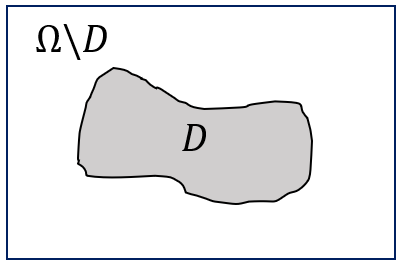
\includegraphics[width=0.4\linewidth]{images/sample-domain.png}
			\caption{ตัวอย่าง โดเมนต่อเติม}
		\end{figure}
		ซึ่งสำหรับปัญหาการต่อเติมภาพโทนสีเทานั้น จะเรียกพื้นที่ซึ่งต้องการต่อเติมว่า โดเมนต่อเติม (inpainting domain) โดย $D$ เป็นโดเมนซึ่ง $D \subset \Omega$ 
		
		โดยการต่อเติมภาพเฉดเทานี้ จะใช้การแปรผันรวม (total variation) ซึ่งถูกคิดค้นโดย Chan และ Shen \cite{ref:rof-inpaint-chan-shen} ซึ่งประยุกต์มาจากการแปรผันรวมเพื่อกำจัดสัญญาณรบกวนบนตัวแบบ ROF \cite{ref:ROF-template}
		
		ได้ว่าจะสามารถหาภาพที่ถูกต่อเติมอย่างเหมาะสม $u$ จะสามารถหาได้จาก
		
			$$\min_{u} \{ \mathcal{J}(u)= \lambda \mathcal{D}(u,f)+  \mathcal{R}(u) \}$$
		
		ซึ่ง $ \mathcal{D} $ คือพจน์สำหรับวัดค่าเหมาะสม เพื่อไม่ให้ภาพก่อนต่อเติมและหลังจากต่อเติมมีความแตกต่างกันมากเกินไป $ \mathcal{R} $ คือพจน์สำหรับการต่อเติมภาพ และ $ \lambda $  คือเปนพารามิเตอรเร็กกิวลารไรซเซชัน (regularization parameter) สำหรับกำหนดปริมาณของสัญญาณรบกวนที่ตองการกำจัดออก 
		
		% ทำการ proposs ไม่ใช่แก้
		โดย Chan และ Shen ได้ทำการแก้ปัญหาการแปรผัน (variational problem) ได้ว่า
		
		$$\min_{u} \{ \mathcal{J}(u) = \frac{\lambda}{2} \int_{\Omega \textbackslash D} (u-z)^2 d\Omega +  \int_{\Omega}  |\bigtriangledown u|  d\Omega \}$$
	
		ซึ่งเมื่อทำให้ได้สมการออยเลอร์ลากรางซ์ สำหรับ fuctional $\mathcal{J}$ คือ 
		
		$$ \left \{ \begin{array}{ll}  - \bigtriangledown \cdot  \Big( \frac{\bigtriangledown u}{|\bigtriangledown u|} \Big) + \lambda (u-z) = 0  & \hspace{1cm} x \in \Omega = (0,n)^2 \\ \frac{\partial u}{\partial n} = 0 & \hspace{1cm} x \in \partial \Omega \end{array} \right . $$
		
		สำหรับ $\mathbf{x} \in \Omega$ ได้ว่า $\lambda$ ถูกกำหนดโดย
		
		% ควรไปอยู่ด้านบน
		$$ \lambda(\mathbf{x}) \left \{ \begin{array}{ll}  \lambda & \mathbf{x} \in \Omega \textbackslash D \\ 0 &\mathbf{x} \in D  \end{array} \right . $$
		
		จะเห็นได้ว่าเป็นสมการออยเลอร์ ลากรางซ์ดังกล่าวเป็น สมการอนุพันธ์ย่อยไม่เป็นเชิงเส้น จึงสามารถใช้วิธีเชิงตัวเลขด้วยวิธีต่างๆ ได้ดังนี้
		
		วิธีการ Explicit Time Marching  \cite{ref:ExplicitTimeMarching}  โดยแนวคิดของวิธีการนี้คือการแนะนําตัวแปรเวลาสังเคราะห์ (time artificial variable) จากนั้นหาคําตอบแบบสภาวะคงตัว (steady-state solution) ของสมการเชิงอนุพันธ์ย่อยไม่เป็นเชิงเส้นที่ขึ้นอยู่กับเวลา และเพื่อจะแก้ความไม่เป็นเชิงเส้นของสมการเชิงอนุพันธ์ย่อย จะสามารถใช้รูปแบบที่ชัดแจ้งของออยเลอร์ (Euler's explicit scheme) ที่กำหนดโดย
		$$
		u(\mathbf{x},t_{k+1})=u(\mathbf{x},t_{k})+\tau\left(\nabla\cdot\left(\frac{\nabla u ( \mathbf{x},t_k)}{\lvert \nabla u ( \mathbf{x},t_k) \rvert }\right) + \lambda(\mathbf{x})(u ( \mathbf{x},t_k)-z(\mathbf{x})) \right)
		$$
		แต่เนื่องจากเมื่อ $\lvert \nabla u ( \mathbf{x},t_k) \rvert = 0 $ จะทำให้ไม่สามารถคำนวณได้ เนื่องจากหารด้วย 0 ไม่ได้ จึงกำหนดให้ $\lvert \nabla u ( \mathbf{x},t_k) \rvert = \sqrt{u_x^2+u_y^2 + \beta}$ สำหรับ $\beta > 0$ และ $\beta$ มีค่าใกล้ 0 เพื่อหลีกเลี่ยงเหตุการณ์ดังกล่าว
		
		โดยเมื่อ $\tau>0$ แทนขั้นเวลา (time step) ที่ได้จากการดิสครีตไทซ์โดเมนเวลา $[0,\infty)$ ซึ่งเห็นได้ว่าวิธีการเชิงตัวเลขดังกล่าวข้างต้นนั้นง่ายในการคํานวณ แต่การลู่เข้าสู่คําตอบที่เหมาะสมของปัญหา เชิงแปรผันค่อนข้างช้ามากเนื่องจากต้องใช้ $\tau$ ที่มีขนาดเล็กในการทำให้ลำดับของคำตอบลู่เข้า 
		
		% บอกว่าอยากได้ beta น้อยๆ แต่มีปัญหาอย่างไร
		วิธีการทำซ้ำแบบ Fixed Point \cite{ref:FixpointSolver} จะทำการแบ่งการทำซ้ำออกเป็น  2 ชั้น เรียกชั้นในกับชั้นนอก โดยการทำซ้ำชั้นใน เป็นการทำซ้ำแบบ Gauss-seidel เพื่อให้หาค่า u เป็นลำดับถัดไป จากนั้นชั้นนอกจะเป็นการทำซ้ำแบบตรึงจุด (fixed point) เพื่อให้ค่า $u$ ลู่เข้าสู่ค่าที่ต้องการ 
		
		ซึ่งการทำซ้ำชั้นในจะหาค่า $u$ จากการใช้ Gauss-Seidel กับสมการ
		$$
		- \nabla\cdot\left(\frac{\nabla u^{[v+1]}}{{\lvert \nabla u \rvert}^{[v]} }\right) + \lambda(u^{[v+1]}-z)  = 0
		$$
		
		โดยที่ $v = 0,1,2,... $ ซึ่งคือค่าของจำนวนครั้งในการทำชั้นนอกที่ถูกทำไป
		
		และเช่นเดียวกับวิธี Explicit Time Marching เนื่องจากวิธีนี้เมื่อ $\lvert \nabla u ( \mathbf{x},t_k) = 0\rvert $ จะทำให้ไม่สามารถคำนวณได้ เนื่องจากไม่สามารถหารด้วย 0 ได้ จึงกำหนดให้ $\lvert \nabla u ( \mathbf{x},t_k) \rvert = \sqrt{u_x^2+u_y^2 + \beta}$ สำหรับ $\beta > 0$ และ $\beta$ มีค่าใกล้ 0 เพื่อหลีกเลี่ยงเหตุการณ์ดังกล่าว
		
		ซึ่งทั้งวิธี Explicit Time Marching และวิธี Fixed Point จำเป็นต้องเพิ่ม $\beta$ เพื่อหลีกเลี่ยงการหารด้วย 0 ซึ่งจะทำให้เกิดค่าคลาดเคลื่อน  จึงได้มีการสร้างวิธี Split Bergman สำหรับแก้ปัญหานี้
		
		%บอกจากจุดเริ่มต้นของปัญหา ต้องการกำจัด beta ที่ทำให้คลาดเคลื่อน
		วิธี Split Bergman \cite{ref:splitbergman-inpaint} โดยวิธีการนี้คือการแยกส่วนการดำเนินการ (spliting) และใช้การทำซ้ำ Bergman (bergman iteration)  โดยวิธีนี้จะเป็นการแก้ปัญหาการแปรผัน โดยการเพิ่มตัวแปร $w$ ในการแก้ปัญหา ซึ่งจะได้ปัญหาการแปรผันดังต่อไปนี้แทน
		
			$$\min_{u} \{ \mathcal{J}(u) = \frac{\lambda}{2} \int_{\Omega \textbackslash D} (u-z)^2 d\Omega +  \int_{\Omega}  |\bigtriangledown w|  d\Omega + \frac{\theta}{2} \int_{\Omega} (w - \bigtriangledown u + b) d\Omega \}$$
			
			โดยเมื่อเพิ่มตัวแปร $w$ สำหรับช่วยใจการคำนวณแล้ว จะมีพจน์ $ \int_{\Omega}  |\bigtriangledown w|  d\Omega$ เพื่อบีบบังคับให้ $w$ ไม่เปลี่ยนแปลงผลของคำตอบ, $\theta$ คือค่าบวกใดๆ ซึ่งเกี่ยวข้องกับความแรงของการต่อเติมซึ่งไม่ควรเล็กหรือใหญ่เกินไปเพื่อให้สามารถลู่เข้าได้ดี $b$ คือตัวแปรช่วยสำหรับการทำซ้ำ Bergman ซึ่งปัญหาดังกล่าวสามารถแบ่งปัญหาได้เป็น 2 ส่วนคือ
			
			ปัญหาย่อย $w$ โดยการคงค่า $u$ ไว้จะได้ว่าปัญหาย่อยคือ
			$$\min_{u} \{ \mathcal{J}(u) =  \int_{\Omega}  |\bigtriangledown w|  d\Omega + \frac{\theta}{2} \int_{\Omega} (w - \bigtriangledown u + b) d\Omega \}$$
			
			ซึ่งเมื่อทำการแก้ปัญหาย่นอนี้แล้วจะได้ว่า
			
				$$ w_{i,j} = \frac{\bigtriangledown u_{i,j}  + b_{i,j} }{ | \bigtriangledown u_{i,j}  + b_{i,j} | } max \{  | \bigtriangledown u_{i,j}  + b_{i,j} | - \frac{1}{\theta} , 0\} $$
				
			ปัญหาย่อย $u$ โดยการคงค่า $w$ ไว้จะได้ว่าปัญหาย่อยคือ

				$$\min_{u} \{ \mathcal{J}(u) = \frac{\lambda}{2} \int_{\Omega \textbackslash D} (u-z)^2 d\Omega + \frac{\theta}{2} \int_{\Omega} (w - \bigtriangledown u + b) d\Omega \}$$
				
			ซึ่งเมื่อทำการแก้ปัญหาย่อยนี้แล้วจะได้ว่า
			$$ \frac{1}{\theta}\lambda u - \bigtriangleup u = \frac{1}{\theta} \lambda z - \bigtriangledown \cdot (w-b) $$
			
			เราจะประมาณคำตอบนี้โดยการใช้ หนึ่งรอบ Gauss-Seidel ต่อหนึ่งรอบการทำซ้ำของ Bergman ซึ่งปัญหาย่อยจะถูกแก้หนึ่งครั้ง ต่อหนึ่งรอบ bergman iteration แต่ทั้งนี้การทำซ้ำ Gauss-Seidel หลายครั้ง จะทำให้การแก้ปัญหาย่อยมีความแม่นยำขึ้น
			ส่วนตัวแปรช่วย $b$ มีค่าเริ่มต้นเป็น 0 จากนั้นทำการปรับค่าโดย
			
			$$ b^{k+1} = b^k  + \bigtriangledown u - w $$
						
			จึงได้ว่าวิธีการ Split Bergman มีการทำงานในภาพรวมเป็นดังนี้
			
			
			
			\begin{algorithm}[H]
				\begin{framed}
					initialization $u = 0, d = 0, b = 0$\\
					\While{ $|| u_{cur} - u_{prev} ||_2 > Tol$}{
						Solve the $w$ subproblem \\
						Solve the $u$ subproblem \\
						$ b = b + \bigtriangledown u - w$
					}
				\end{framed}
			\end{algorithm}
			
			
			
			โดยการทำซ้ำนี้จะกระทำจนกระทั่ง นอร์ม L2 ระหว่างรอบปัจจุบันต่างกับรอบก่อนหน้าไม่เกินค่า Tol ที่กำหนดไว้หรือจำนวนรอบการทำซ้ำมากจนถึงจุดสิ้นสุดที่เพียงพอที่จะให้ลู่เข้าซึ่งไม่ควรใหญ่เกินไปเพื่อไม่ให้เสียเวลาประมวลผลจนนานเกินไป 

			โดยผลการต่อเติมภาพจากทั้ง 3 วิธีข้างต้น สำหรับการกำหนดรอบการทำซ้ำไม่เกิน 1000 รอบและค่านอร์ม L2 ภาพปัจจุบันและภาพก่อนหน้าต่างกันไม่เกิน 0.0001 ได้ผลลัพธ์ดังนี้
			
			\begin{figure}[H]
				\centering
				\begin{subfigure}{0.3\linewidth}
					\centering
					
\includegraphics[width=0.3\linewidth]{images/grayscale_inpaint/original.png}
					\caption{ภาพต้นฉบับ}
				\end{subfigure}
				\begin{subfigure}{0.3\linewidth}
					\centering
					
\includegraphics[width=0.3\linewidth]{images/grayscale_inpaint/toinapint.png}
					\caption{ภาพที่ต้องการทำการต่อเติม}
				\end{subfigure}
			\begin{subfigure}{0.3\linewidth}
				\centering
					
\includegraphics[width=0.3\linewidth]{images/grayscale_inpaint/inpaintdomain.png}
				\caption{โดเมนต่อเติม}
			\end{subfigure}
		\begin{subfigure}{0.3\linewidth}
			\centering
			
\includegraphics[width=0.3\linewidth]{images/grayscale_inpaint/result_timemarch.png}
			\caption{ภาพจากวิธี Explicit Time Marching ใช้เวลา 3.10 วินาที PSNR 19.6733}
		\end{subfigure}
		\begin{subfigure}{0.3\linewidth}
			\centering
			
\includegraphics[width=0.3\linewidth]{images/grayscale_inpaint/result_fixpoint.png}
			\caption{ภาพจากวิธี Fixed Point ใช้เวลา 6.93 วินาที PSNR 42.6631}
		\end{subfigure}
		\begin{subfigure}{0.3\linewidth}
			\centering
			
\includegraphics[width=0.3\linewidth]{images/grayscale_inpaint/result_splitbergman.png}
				\caption{ภาพจากวิธี Split Bergman ใช้เวลา 1.86 วินาที PSNR 44.4275}
		\end{subfigure}
		\end{figure}
			
			จากการทดลองจะเห็นว่าวิธีการ Split Bergman ได้ผลลัพธ์ที่ดีที่สุด จึงได้มีความสนใจที่จะศึกษาวิธี Split Bergman เป็นลำดับถัดไป
			
			
			% ต้องบอกว่า PSNR SSIM RMSE มาอย่างไร
			
			\subsection{วิธีการทางคณิตศาสตร์สำหรับการต่อเติมภาพด้วยการแปรผันบนภาพสี} 

			สำหรับการต่อเติมภาพเชิงแปรผันซึ่งเป็นภาพสีในระบบ RGB จะพิจารณา
			
			$$ u = (u_1,u_2,u_3)^{\top} : \Omega  \rightarrow V^3 $$

			\noindent เมื่อ $\u=(u_1,u_2,u_3)$ โดยที่ $u_1,u_2,u_3: \Omega  \rightarrow V$ แทนภาพเฉดสีแดง สีเขียว และสีน้ำเงินของ $u$ ตามลำดับ จะสามารถปรับปรุงตัวแบบ ROF ได้ดังนี้
			
			$$\min_{u} \{ \mathcal{J}(u)= \lambda \mathcal{\bar{D}}(u,z)+  \mathcal{\bar{R}}(u) \}$$
			
			โดยที่ $\mathcal{\bar{D}}$ เป็นพจน์วัดค่าเหมาะสมเพื่อไม่ให้ภาพก่อนการต่อและหลังต่อเติมต่างกันมาเกินไปซึ่ง
			\begin{align*}
			\mathcal{\bar{D}}(\boldsymbol{u},\boldsymbol{z})  &= \underset{l=1}{\overset{3}{\sum}}\mathcal{D}(u_l,z_l) \\
			&= \frac{1}{2}\int_{\Omega}^{}(u_1 - z_1)^2 d\Omega + \frac{1}{2}\int_{\Omega}^{}(u_2 - z_2)^2 d\Omega + \frac{1}{2}\int_{\Omega}^{}(u_3 - z_3)^2 d\Omega
			\end{align*}
			
			และ $ \mathcal{\bar{R}} $ คือพจน์สำหรับการต่อเติมภาพ 
			
			\begin{align*}
			\mathcal{\bar{R}}(\boldsymbol{u}) &= \underset{l=1}{\overset{3}{\sum}}\mathcal{R}(u_l) = \int_{\Omega}^{}\lvert\nabla u_1 \rvert d\Omega + \int_{\Omega}^{}\lvert\nabla u_2 \rvert d\Omega + \int_{\Omega}^{}\lvert\nabla u_3 \rvert d\Omega
			\end{align*}
			
			ซึ่งงานนี้ได้สนใจที่จะนำวิธี Split Bergman มาประยุกต์ใช้กับปัญหาเชิงแปรผัน จึงแนะนำเวกเตอร์เสริม $w_1, w_2, w_3$ พร้อมทั้งตัวแปรสำหรับการทำซ้ำ Bregman $b_1, b_2, b_3$ และตัวแปรช่วย $\theta_1, \theta_2, \theta_3 > 0 $ เพื่อแก้ปัญหาเชิงแปรผัน ซึ่งจะได้ปัญหาเชิงแปรผันเป็น
			
			$$ 
			\min_{u} \{\bar{\mathcal{J}}= \lambda \mathcal{\bar{D}}(u,z) +  \underset{l=1}{\overset{3}{\sum}} \int_{\Omega}^{}|\boldsymbol{w_l}|d\Omega
			+ \frac{\theta_l}{2} \underset{l=1}{\overset{3}{\sum}}\int_{\Omega}^{}(\boldsymbol{w_l} - \nabla u_l - \boldsymbol{b_l})^{2}d\Omega\}
			$$
			
			% เขียน functional เป็นเฉพาะ w เท่านั้น ไม่ต้องพูดอะไรมาก ยังไม่ต้องบง gauss-siedel เอา gauss-seidel ออกไปก่อน
			
			
			ปัญหาย่อย $w$ โดยการคงค่า $u$ ไว้จะได้ว่าปัญหาย่อยคือ
			
			$$ 
			\min_{u} \{\bar{\mathcal{J}}= \underset{l=1}{\overset{3}{\sum}} \int_{\Omega}^{}|{w_l}|d\Omega
			+ \frac{\theta_l}{2} \underset{l=1}{\overset{3}{\sum}}\int_{\Omega}^{}({w_l} - \nabla u_l - {b_l})^{2}d\Omega\}
			$$
			
			ซึ่งเมื่อทำการแก้ปัญหาย่อยนี้จะได้คำตอบที่แม่นตรงคือ
			
			$$ w_{l_{i,j}} = \frac{\bigtriangledown u_{l_{i,j}}  + b_{l_{i,j}} }{ | \bigtriangledown u_{l_{i,j}}  + b_{l_{i,j}} | } max \{  | \bigtriangledown u_{l_{i,j}}  + b_{l_{i,j}} | - \frac{1}{\theta} , 0\} \hspace{1cm}  \hspace{0.1cm} l = 1,2,3$$ 
			
			
			ปัญหาย่อย $u$ โดยการคงค่า $w$ ไว้จะได้ว่าปัญหาย่อยคือ
			
				$$ 
			\min_{u} \{\bar{\mathcal{J}}= \lambda \mathcal{\bar{D}}(u,z) + \frac{\theta_l}{2} \underset{l=1}{\overset{3}{\sum}}\int_{\Omega}^{}(\boldsymbol{w_l} - \nabla u_l - \boldsymbol{b_l})^{2}d\Omega\}
			$$
			
			ซึ่งเมื่อทำการแก้ปัญหาย่อยนี้แล้วจะได้ระบบสมการออยเลอร์ลากรางจ์คือ
			
			$$ \frac{1}{\theta}\lambda u_1 - \bigtriangleup u_1 = \frac{1}{\theta} \lambda z_1 - \bigtriangledown \cdot (w_1-b_1) $$
			
			$$ \frac{1}{\theta}\lambda u_2 - \bigtriangleup u_2 = \frac{1}{\theta} \lambda z_2 - \bigtriangledown \cdot (w_2-b_2) $$
			
			$$ \frac{1}{\theta}\lambda u_3 - \bigtriangleup u_3 = \frac{1}{\theta} \lambda z_3 - \bigtriangledown \cdot (w_3-b_3) $$
			
			ซึ่งเมื่อแก้ระบบสมการดังกล่าวด้วยวิธี Gauss-seidel แล้วจะนำค่าที่ได้มาเปลี่ยนค่าตัวแปร $b$ โดยที่
			
			$$ b_{l}^{k+1} = b_{l}^k  + \bigtriangledown u_{l} - w_{l} \hspace{1cm}  \hspace{0.1cm} l = 1,2,3 $$
			
			ซึ่งจากวิธีการ Split Bergman สำหรับภาพสี จะได้ภาพผลลัพธ์ดังนี้
			
			\begin{figure}[H]
				\centering
				\begin{subfigure}{0.4\linewidth}
					\centering
					
\includegraphics[width=0.4\linewidth]{images/color_inpaint/original.png}
					\caption{ภาพต้นฉบับ}
				\end{subfigure}
				\begin{subfigure}{0.4\linewidth}
					\centering
					
\includegraphics[width=0.4\linewidth]{images/color_inpaint/toinpaint.png}
					\caption{ภาพที่ต้องการทำการต่อเติม}
				\end{subfigure}
				\begin{subfigure}{0.4\linewidth}
					\centering
					
\includegraphics[width=0.4\linewidth]{images/color_inpaint/inpaintdomain.png}
					\caption{โดเมนต่อเติม}
				\end{subfigure}
				\begin{subfigure}{0.4\linewidth}
					\centering
					
\includegraphics[width=0.4\linewidth]{images/color_inpaint/result_splitbergman.png}
					\caption{ภาพจากวิธี Split Bergman ใช้เวลา 6.72 วินาที PSNR 37.2374}
				\end{subfigure}
			\end{figure}
			
			\subsection{การประยุกต์ใช้สำหรับซ่อมแซมภาพวาดศิลปะไทย}
			
			\hspace{0.85cm}เนื่องจากการต่อเติมภาพด้วยการแปรผันจะสนใจที่ความต่อเนื่องของโครงสร้างทางเรขาคณิต ซึ่งวิธีการต่อเติมภาพรูปภาพด้วยการแปรผันมักจะให้ผลลัพธ์ได้ดีกับรูปภาพที่ราบเรียบเป็นช่วง (piecewise smooth image) \cite{ref:defination-of-variation-inpaint}  ซึ่งภาพวาดศิลปะไทยนั้น เป็นภาพซึ่งมีลักษณะราบเรียบเป็นช่วงจึงเหมาะสำหรับใช้แม่แบบวิธี ROF สำหรับการต่อเติมภาพ เนื่องจากในปัจจุบันนี้ยังมีงานศิลปะไทยเก่าจำนวนมากที่ต้องการได้รับการซ่อมแซมจึงเป็นการช่วยให้จิตรกรผู้มีหน้าที่ซ่อมแซมภาพ สามารถเห็นตัวอย่างภาพที่ผ่านการต่อเติม เพื่อให้จิตรกรสามารถวางแผนในการซ่อมแซมได้ หรือการเข้าชมพิพิธภัณฑ์ ก็อาจพัฒนาเป็นแอปพลิเคชันสำหรับโทรศัพท์มือถือ ที่สามารถใช้ส่องภาพงานศิลปะและแสดงศิลปะที่สมบูรณ์ขึ้นมาทางหน้าจอได้
			\begin{figure}[H]
				\centering
				\begin{subfigure}{0.4\linewidth}
					\centering
					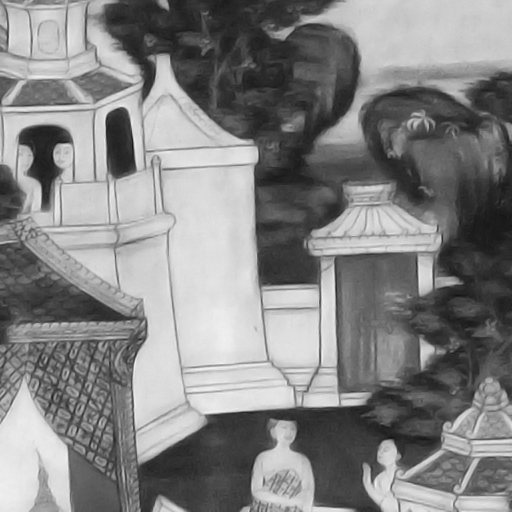
\includegraphics[width=0.4\linewidth]{images/show_peicewise/thaiart_gray.png}
					\caption{ภาพศิลปะไทยซึ่งเป็นเฉดสีเทา}
				\end{subfigure}
				\begin{subfigure}{0.4\linewidth}
					\centering
					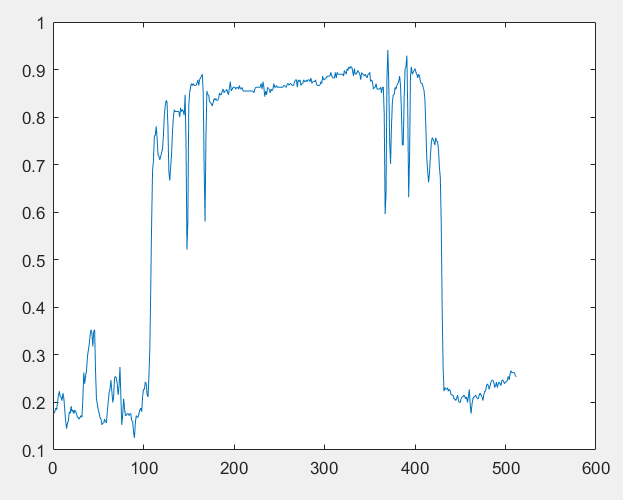
\includegraphics[width=0.4\linewidth]{images/show_peicewise/thaiart_is_piecewise.png}
					\caption{ความเข้มของสีบริเวณคอลัมม์ที่ 200}
				\end{subfigure}				
			\end{figure}
			โดยจากตัวอย่างจะเป็นภาพวาด จิตรกรรม อุโบสถวัดคงคาราม ขนาด 512x512 ซึ่งถูกปรับให้เป็นเฉดสีเทา เมื่อนำข้อมูลความเข้มของสีบริเวณคอลัมม์ที่ 200 มาเขียนกราฟจะเห็นว่าบริเวณจุดที่ 100 และจุดที่ 420 มีความแตกต่างของความเข็มอย่างชัดเจน โดยแบ่งเป็นช่วง (0,100), (100,420) และ (420,512) ซึ่งมีลักษณะราบเรียบเป็นช่วงนั่นเอง
				
			% คืออะไร ต้องการ solve แบบไหน สรุปว่า ผู้วิจัยต้องการวิธีเชิงตัวเลขเพื่อประยุกต์สำหรับ ??? 
			\subsection{กาประยุกต์ใช้สำหรับการลบคำบรรยายบนอนิเมะ}
			\hspace{0.85cm}อนิเมะคือวิดีโอภาพวาดการ์ตูนสไตล์ญี่ปุ่น ซึ่งภาพวาดสไตล์ของอนิเมะเองก็เป็นภาพแบบราบเรียบเป็นช่วงจึงเหมาะกับการใช้แม่แบบวิธี ROF สำหรับการต่อเติมภาพ	ซึ่งอนิเมะนั้นเนื่องจากผ่านการแปลภาษามาแล้ว ในบางครั้งจะมีคำบรรยายแบบแข็งติดมาด้วย ซึ่งบทบรรยายแบบแข็งนั้นไม่สามารถเปิดและปิดได้ เมื่อผ่านการให้เสียงใหม่แล้วก็จะมีบทบรรยายนั้นติดมาด้วย จึงเหมาะที่จะประยุกต์ใช้ในการลบทบรรยายออก

			สำหรับการต่อเติมภาพนั้น โดยปกติจะเป็นต้องหาโดเมนต่อเติมด้วยตัวเองซึ่งสามารถทำได้สำหรับภาพ  1 ภาพ แต่สำหรับไฟล์วิดีโออนิเมะนั้น ส่วนใหญ่จะมีภาพจำนวน 24 ภาพต่อวินาที ซึ่งนั่นหมายความว่าการจะหาโดเมนต่อเติมด้วยตัวเองสำหรับ 24 ภาพต่อวินาทีเป็นเรื่องยาก การที่จะหาโดเมนต่อเติมซึ่งเป็นในส่วนคำบรรยายนั้นจึงเป็นเรื่องยาก จึงเป็นอีกความท้าทายที่จะต้องหาโดเมนต่อเติมแบบอัตโนมัติให้ได้
			
			\begin{figure}[H]
				\centering
				\begin{subfigure}{0.4\linewidth}
					\centering
					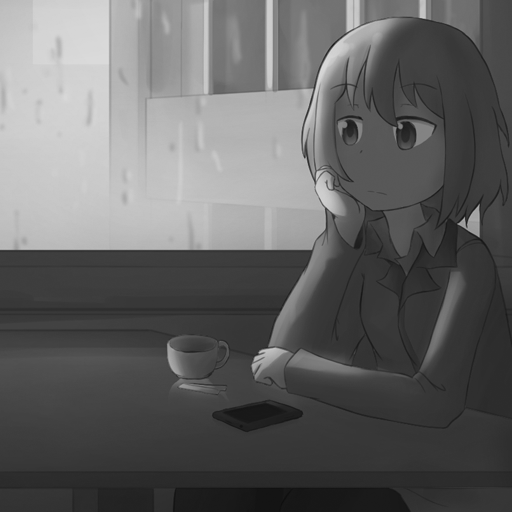
\includegraphics[width=0.4\linewidth]{images/show_peicewise/anime_gray.png}
					\caption{ภาพอนิเมะซึ่งเป็นเฉดสีเทา}
				\end{subfigure}
				\begin{subfigure}{0.4\linewidth}
					\centering
					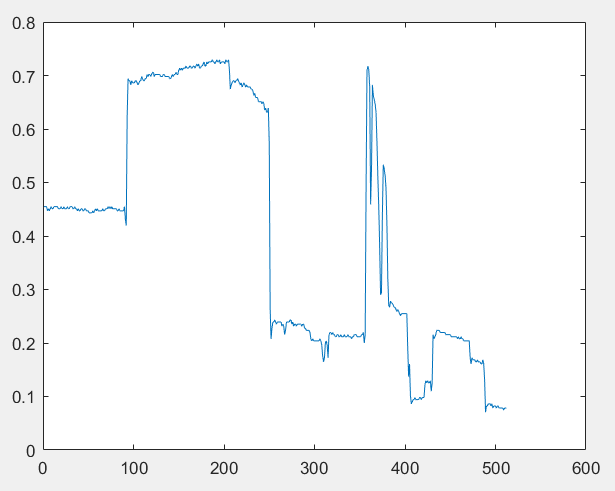
\includegraphics[width=0.4\linewidth]{images/show_peicewise/anime_is_piecewise.png}
					\caption{ความเข้มของสีบริเวณคอลัมม์ที่ 256}
				\end{subfigure}				
			\end{figure}
			โดยจากตัวอย่างจะเป็นภาพอนิเมะ ขนาด 512x512 ซึ่งถูกปรับให้เป็นเฉดสีเทา เมื่อนำข้อมูลความเข้มของสีบริเวณคอลัมม์ที่ 256 มาเขียนกราฟจะเห็นว่าบริเวณจุดที่ 100,250,350,400,420,480 มีความแตกต่างของความเข็มอย่างชัดเจน โดยแบ่งเป็นช่วง (0,100), (100,250), (250,350), (400,420)  และ (480,512) ซึ่งมีลักษณะราบเรียบเป็นช่วงนั่นเอง
		
		% สรุปว่าโครงกานี้จะทำอะไร สรุปเอาให้ชัด 
		% ผู้วิจัยต้องการพัฒนาวิธีเชิงตัวเลขสำหรับ ...
		
		% ====================================
\section{Objective}
วัตถุประสงค์ของโครงการวิจัยมีดังต่อไปนี้
\begin{description}
	\item[(1)]	 ศึกษาวิธีการแปรผันและวิธีการเชิงตัวเลขที่มีประสิทธิภาพเพื่อเติมข้อมูลที่ขาดหายในภาพหรือวิดีโอ
	\item[(2)] สร้างวิธีการเชิงตัวเลขใหม่สำหรับซ่อมแซมภาพศิลปะไทยและลบบทบรรยายออกจากอนิเมะ
	\item[(3)] นำวิธีการที่สร้างขึ้นเพื่อซ่อมแซมภาพไทย และลบบทบรรยายในอนิเมะ
\end{description}

% เราต้องการต่อเติมภาพสี และซ่อมแซมศิลปะไทย
% ตัว piceewise เล่ายาว
% ถ้าไม่จำเป็น ไม่ต้องลงประเด็นใหม่ พร้อมกว่านี้ค่อยทำ
% ปัญหาชัดเจนไหม สังเคราะห์ข้อมูลอย่างไร การประมวลผลข้อมูล

\section{Scope of Study}
% จะใช้ PSNR SSIM ของภาพ ของวิดีโออย่างไร
ขอบเขตของโครงงานมีดังต่อไปนี้
\begin{description}
\item[(3.1)] ภาพศิลปะที่ใช้ศึกษา เป็นภาพจิตรกรรมฝาผนังไทย ที่อยู่ภายใต้เว็บ Wikipedia.org ซึ่งได้รับการอนุญาตให้ใช้งานแบบ Creative Commons หรือแบบ Public Domain
\item[(3.2)] วิดีโอที่ใช้ศึกษาเป็นวิดีโอประเภทอนิเมะ โดยศึกษากับไฟล์อนิเมะที่ใช้ Color space แบบ RGB เท่านั้น
\item[(3.3)] บทบรรยายที่ใช้ทดสอบ จะถูกล้อมรอบไว้ด้วยสีดำ ขนาดความหนาขนาดไม่น้อยกว่า 5 พิกเซล
\item[(3.4)] วิดีโอที่ใช้ศึกษาขนาดไม่เกิน 1920x1080
\item[(3.5)] คอมพิวเตอร์ที่ใช้ทดลองใช้หน่วยประมวลผล I7-6700HQ ใช้การ์ดจอ Nvidia GTX 960M แรม 16GB ฮาร์ดดิกส์แบบ SSD
\end{description}

\section{Methodology}
วิธีการมีดังต่อไปนี้
\begin{description}
	\item[(4.1)] ศึกษาการคณิตศาสตร์ต่อเติมข้อมูลที่ขาดหายบนรูปภาพ
	\item[(4.2)] พัฒนาวิธีการเชิงตัวเลขสำหรับการซ่อมแซมรูปภาพ
	\item[(4.3)] ทดสอบวิธีการเชิงตัวเลขที่พัฒนาขึ้นโดยโปรแกรมคอมพิวเตอร์บนภาพสังเคราะห์
	\item[(4.4)] อภิปรายผลที่ได้จากการทดลองเชิงตัวเลข
	\item[(4.5)] สรุปผลการดำเนินงานวิจัยและจัดทำรูปเล่มฉบับสมบูรณ์
\end{description}
\section{Time Periods}
แผนการดำเนินงานตลอดทั้งโครงการสามารถสรุปได้โดยย่อจากตารางต่อไปนี้
\begin{center}
	\begin{tabular}[ht]{|l|c|c|c|c|c|c|c|c|c|c|c|c|}
		\hline
		&\multicolumn{12}{c|}{เดือนที่}\\
		\cline{2-13}
		แผนการดำเนินงาน&1&2&3&4&5&6&7&8&9&10&11&12\\
		\hline
		ศึกษาการคณิตศาสตร์ต่อเติมข้อมูลที่ขาดหายบนรูปภาพ&x&x& & & & & & & & & &\\
		พัฒนาวิธีการเชิงตัวเลขสำหรับการซ่อมแซมรูปภาพ& & &x&x& & & & & & & &\\
		ทดสอบวิธีการเชิงตัวเลขที่พัฒนาขึ้นโดยโปรแกรม- & & & & &x&x& & & & & &\\
		คอมพิวเตอร์บนภาพสังเคราะห์ & & & & & & & & & & & &\\
		อภิปรายผลที่ได้จากการทดลองเชิงตัวเลข & & & & & & &x&x& & & &\\
		สรุปผลการดำเนินงานวิจัยและจัดทำรูปเล่มฉบับสมบูรณ์& & & & & & & & &x&x&x&x\\
		\hline
	\end{tabular}
\end{center}




\section{References}

\renewcommand{\section}[2]{} % addition mod: remove reference text
\begin{thebibliography}{}
	% ให้ใส่แบบหลังเปเปอร์
	\bibitem{ref:defination-of-inpaint} 
	Furht B., "Image Inpainting", Encyclopedia of Multimedia, pp. 315-316, 2006. .\url{https://doi.org/10.1007/0-387-30038-4_98}
	
	\bibitem{ref:rof-inpaint-chan-shen} 
	T.F. Chan, J. Shen, “Mathematical models of local non-texture inpaintings”, SIAM Journal on Applied Mathematics, vol. 62, no. 3, pp. 1019–1043, 2001. \url{http://www.jstor.org/stable/3061798}
	
	\bibitem{ref:ROF-template} 
	Leonid I. Rudin, Stanley Osher, Emad Fatemi, "Nonlinear total variation based noise removal algorithms", Physica D: Nonlinear Phenomena, Volume 60, Issues 1–4, pp. 259-268, 1992. \url{https://doi.org/10.1016/0167-2789(92)90242-F}
	
	\bibitem{ref:ExplicitTimeMarching} 
	A. Marquina, S. Osher, "Explicit algorithms for a new time dependent model based on level set motion for nonlinear deblurring and noise removal",  
	SIAM Journal on Scientific Computing, vol. 22 issue 2, 387–405. 2006.  \url{https://doi.org/10.1137/S1064827599351751}
	
	\bibitem{ref:FixpointSolver}
	C.R. Vogel and M.E. Oman,"Iterative methods for total variation denoising", SIAM Journal on Scientific Computing. vol. 17, pp. 227-238, 1996.
	
	\bibitem{ref:splitbergman-inpaint}
	   Pascal Getreuer, Total Variation Inpainting using Split Bregman, Image Processing On Line, 2 (2012), pp. 147–157. \url{https://doi.org/10.5201/ipol.2012.g-tvi}
	
	
	\bibitem{ref:defination-of-variation-inpaint}
	Fidaner, Işık Barış. “A Survey on Variational Image Inpainting , Texture Synthesis and Image Completion.” (2007). \url{https://www.semanticscholar.org/paper/_/36f4d32ce45f72091510ab4d4d1cc3bf81ffe879}
	
\end{thebibliography}


\end{document}
	
	
	
	